
% MAIN is the main file for the draft 
% Author: Stephan Gahima
% paper-draft-tex/templates

% ----------------------------------------------------------
%                        PREAMBLE
% ----------------------------------------------------------
%
%	SETUP
%
\documentclass[11pt]{article}
% UTF-8 encoding (https://en.wikipedia.org/wiki/UTF-8)
% !TEX encoding = UTF-8 Unicode
\usepackage[utf8]{inputenc}                		
% Font encoding (http://www.micropress-inc.com/fonts/encoding/t1.htm)
\usepackage[T1]{fontenc}                   		  
\usepackage{lmodern}
\usepackage[inner=2cm, outer=2cm, top=2cm, bottom=3cm]{geometry}   
% ----------------------------------------------------------
% 
%   PACKAGES
%

% Framed and shaded regions that can break across pages
\usepackage{framed} 
% Mathematical miscellaneous
\usepackage{amsmath}
% Mathematical symbols
\usepackage{amssymb}
% Accents. Like \hat{x}, \tilde{x} etc
\usepackage{accents}
% Mathematical notation
\usepackage{fixmath}
% Table formatting
\usepackage{booktabs}
% Tables, and figures placement
\usepackage{float}
% Number formatting
\usepackage{siunitx}
\sisetup{
    round-mode = places,
	round-precision = 3
}
% Reference management
\usepackage{cite} 
% Cross-references, URLS and more with back reference
\usepackage[backref=page]{hyperref}               
\hypersetup{
	colorlinks = false,         % Disable coloured links and anchors 
	pdfauthor = Stephan Gahima,	% Document author, fill in yours
	pdfstartpage = 1,           % PDF opens at page 1
}
% Modify how Backref appears
\renewcommand*{\backref}[1]{}
\renewcommand*{\backrefalt}[4]{{\footnotesize [%
		\ifcase #1 Not cited.%
		\or Cited on page~#2%
		\else Cited on pages~#2%
		\fi%
		]}}
	
% Figures
\usepackage{graphicx}
\usepackage{tikz}
\usepackage{caption}                    
\usepackage[format=hang]{subcaption}    
\newcommand{\subfigsz}{0.4}  

% Include source code
%\usepackage{listings}
% Matlab (http://www.ctan.org/pkg/matlab-prettifier)
\usepackage{matlab-prettifier} 

% ----------------------------------------------------------
%
%   COSTUM COMMANDS
%

% Keywords command
\providecommand{\keywords}[1]
{
	\small	
	\textbf{\textit{Keywords --- }} #1
}

% Mathematics
% Vectors
\renewcommand{\vec}[1]{\mathbold{#1}} 
% Matrices
\newcommand{\mat}[1]{\mathbold{#1}}  

% Typesetting
\newcommand{\refalg}[1]{Algorithm~\ref{#1}}
%\newcommand{\refapp}[1]{Appendix~\ref{#1}}
\newcommand{\refeq}[1]{Equation~\ref{#1}}
\newcommand{\reffig}[1]{Figure~\ref{#1}}
\newcommand{\refsec}[1]{Section~\ref{#1}}
\newcommand{\reftab}[1]{Table~\ref{#1}}

% ----------------------------------------------------------
%                       END OF PREAMBLE
% ----------------------------------------------------------


% Capitalize your title at https://capitalizemytitle.com/
\title{A Template for Your Manuscript Draft} % APA style

\begin{document}
	
	\maketitle
	
	
% ABSTRACT is the file for the abstract
% Author: Stephan Gahima
% paper-draft-tex/templates/src

\begin{abstract}
	This abstract introduces a straightforward and highly customizable LaTeX template tailored for scientific paper drafting. 
	The template provides essential elements such as title, abstract, sections, and bibliography. 
	Its minimalistic approach allows authors to focus on their research findings.
	Researchers can easily customize the layout, font styles, and section headings to align with specific journal or conference guidelines. 
	The user-friendly code makes it accessible to researchers of all levels, from beginners to seasoned LaTeX practitioners. 
	Newcomers can quickly grasp the essentials, while experienced users can efficiently build upon the template to create more complex structures.
	In conclusion, the presented basic and customizable LaTeX template offers a user-friendly solution for drafting scientific papers. 
\end{abstract}
	
	% Add your keywords here
	\keywords{LaTeX, Template, Paper, Drafting}
	
	% introduction.tex
% Introduction section of the manuscript
% Stephan Gahima/paper-draft-tex

\section{Introduction \label{sec:introduction}}
	In~\cite{ACleverResearcher2023}, they show that for researchers is crucial to focus on research findings.
	\reffig{fig:cool-images} shows a relaxed cat. 
	Note that the first author in~\cite{ACleverResearcher2023} loves cats.
	
	\begin{figure}[H]
		\centering
		% You might want to adjust the image, since it does not have axes, labels or fonts
		\includegraphics[height=.5\textwidth]{fig/nice-cat.jpg}
		\caption{
			A relaxed cat picture, saved in JPG format. \href{https://www.pexels.com/photo/orange-tabby-cat-on-brown-knitted-textile-982300/}{Source}.
			\label{fig:cool-images}
		}
	\end{figure}
	
	
% MATERIALS-AND-METHODS is the file for the materials and methods of the paper
% Author: Stephan Gahima
% paper-draft-tex/templates/src

\section{Materials and Methods \label{sec:materials-and-methods}}
    \(\vec{x}\in\mathbb{R}^3\) is a three-dimensional vector, while \(\mat{Y}\in\mathbb{R}^{3\times 6}\) is a three-by-six matrix. 
    The \emph{mass-energy} equation reads
    \begin{equation}
        \label{eq:mass-energy-equivalence}
	    E = m c^2
    \end{equation}

    \refeq{eq:mass-energy-equivalence} is very famous.

	
% RESULTS is the file for the results of the paper
% Author: Stephan Gahima
% paper-draft-tex/templates/src

\section{Results \label{sec:results}}
	In \reftab{tab:alien-visits}, you can see the past and expected visits of Aliens to Earth. 
	
	\begin{table}[H]
		\centering
		\begin{tabular}{llcS}
			\toprule
			Date of Visit & Travel Duration & Landing Location & {Distance Traveled (Km)} \\
			\midrule
			2022-03-15 & 1 year & Area 51, Nevada, USA & \num{450000} \\
			2023-01-08 & 6 months & Giza Pyramid Complex, Egypt & \num{250000} \\
			2023-06-20 & 2 years & The Great Wall of China & \num{802349} \\
			2024-02-12 & 3 months & Machu Picchu, Peru & \num{1500490} \\
			2024-09-30 & 5 years & Mount Kilimanjaro, Tanzania & \num{1200000} \\
			2025-05-18 & 1.5 years & Stonehenge, United Kingdom & \num{600000} \\
			2026-11-02 & 8 months & Mount Everest, Nepal & \num{300000} \\
			2027-08-10 & 4 years & Ayers Rock (Uluru), Australia & \num{1000000} \\
			2028-12-24 & 2.5 years & Taj Mahal, India & \num{700422} \\
			2029-09-03 & 3.5 years & Christ the Redeemer, Brazil & \num{900000} \\
			\bottomrule
		\end{tabular}
		\caption{\href{https://chat.openai.com/}{ChatGPT} generated data about past and expected Alien visits to Earth. \label{tab:alien-visits}}
	\end{table}

	\reffig{fig:cool-images} shows a relaxed cat. 
	Note that the first author in~\cite{ACleverResearcher2023} loves cats.
	
	\begin{figure}[H]
		\centering
		% You might want to adjust the image, since it does not have axes, labels or fonts
		\includegraphics[width=.5\textwidth]{fig/nice-cat.jpg}
		\caption{
			A relaxed cat picture, saved in JPG format. \href{https://www.pexels.com/photo/orange-tabby-cat-on-brown-knitted-textile-982300/}{Source}.
			\label{fig:cool-images}
			}
	\end{figure}
	
	To visualize the sparsity pattern of a matrix \(\mat{S}\in\mathbb{R}^{100\times 100}\) and the classification of the \href{https://en.wikipedia.org/wiki/Iris_flower_data_set}{Fisher's iris dataset}, you can use the Matlab source codes \ref{code:fig2a}-\ref{code:fig2b}. Running these codes will produce the output \reffig{fig:math-stuff}.
	
	\begin{lstlisting}[style=Matlab-editor, caption={Matlab code for \reffig{fig:sparsity}}, label=code:fig2a]
		% Source code for Figure 2a
		 S = sprand(100, 100, .1);
		 f = figure; 
		 spy(S);
	\end{lstlisting}
		
	\begin{lstlisting}[style=Matlab-editor, caption={Matlab code for \reffig{fig:classification}}, label=code:fig2b]
		% Source code for Figure 2b
		load fisheriris.mat; 
		f = figure;
		gscatter(meas(:, 1), meas(:, 2), species, 'rgb', 'osd');
		xlabel('Sepal length');
		ylabel('Sepal width');
	\end{lstlisting}
	
%	% Add reference to the code that produced the figure.
%	\begin{figure}[H]
%		\centering
%		\begin{subfigure}{\subfigsz\textwidth}
%			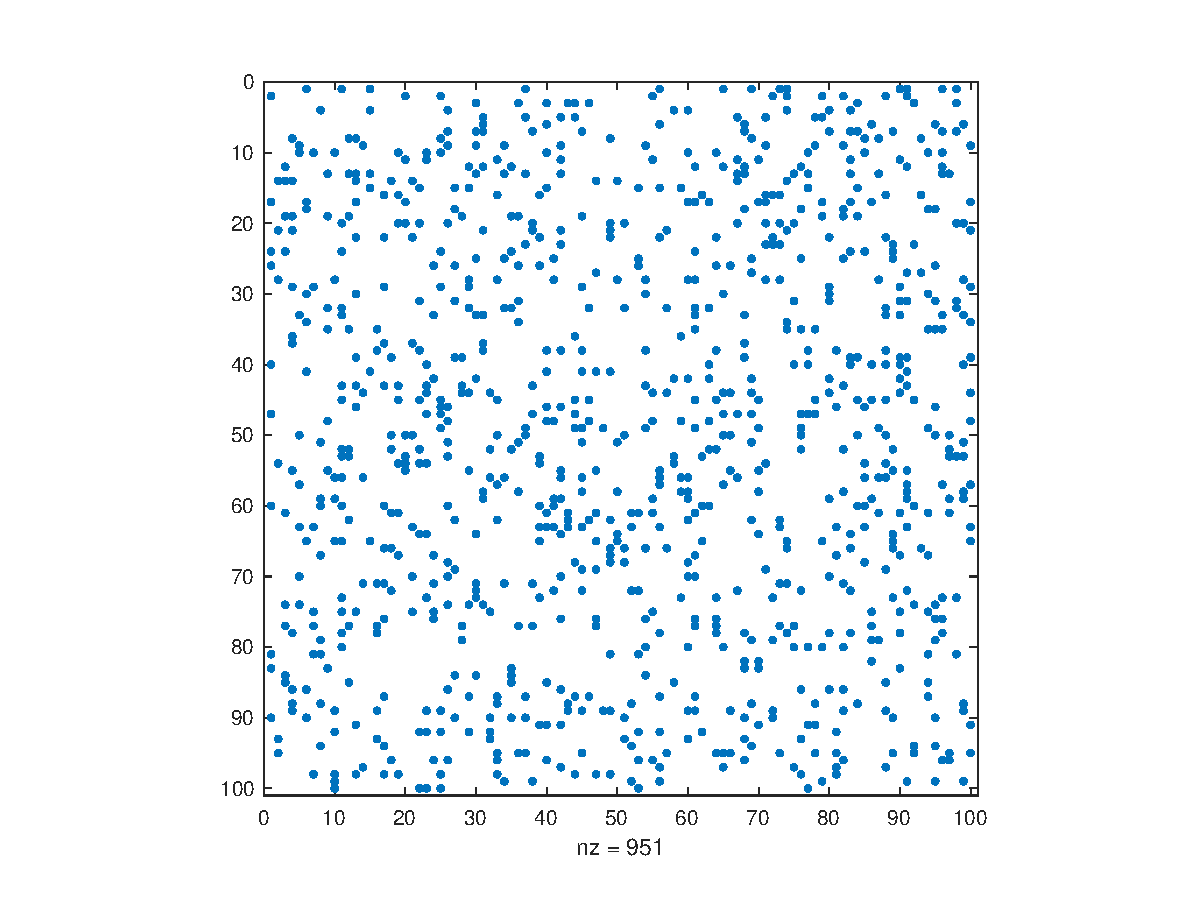
\includegraphics[width=\textwidth]{fig/sparsity.eps}
%			\subcaption{
%				Sparsity pattern of matrix \(\mat{S}\).
%				\label{fig:sparsity}
%			}
%		\end{subfigure}
%		\begin{subfigure}{\subfigsz\textwidth}
%			\includegraphics[width=\textwidth]{fig/classification.pdf}
%			\subcaption{
%				Classification of the Fisher's iris dataset.
%				\label{fig:classification}
%			}
%		\end{subfigure}
%		\caption{EPS (a) and PDF (b) figures. \label{fig:math-stuff}}
%	\end{figure}



	% discussion.tex
% contains the text for the discussion section of the manuscript
% paper-draft-tex/templates/src

\section{Discussion \label{sec:discussion}}
	\refsec{sec:introduction} showed how citation works.
	\ref{sec:materials-and-methods} briefly touched on mathematical notation, and \refsec{sec:results} presented how to format tables and figures.
	In particular, to have nice-looking figures, we recommend using this Matlab function \texttt{ffsp}.
	\refalg{alg:figure-formatting} describes the \texttt{ffsp} procedure.
	


	\bibliographystyle{plain}
	\bibliography{src/bibliography}
	
	\clearpage
	
	\listoffigures
	\listoftables
	\lstlistoflistings
	
\end{document}